\scanpage{21}
\begin{flushright}\begin{minipage}{.54\linewidth}
Descriptions transcendantes de motifs en car $0$ et de catégories de motifs en car. $0$

\figure{\hspace{.16\linewidth}
\begin{tikzpicture}
 \draw[line width=.6pt,line cap=round] (0,0) .. controls (.55,.01) and (1.25,.03) .. (1.72,.14);
\end{tikzpicture}}

doubles réseaux etc
\end{minipage}\end{flushright}

\vspace{1cm}
\figure{\hspace{.15\linewidth}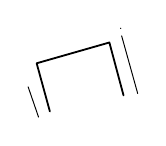
\begin{tikzpicture}[x=.012cm,y=-.012cm,line cap=round,line join=round]
 \draw[line width=.65pt] (24,97) -- (10,46) -- (87,24) -- (102,80);
 \draw[line width=.35pt] (1,71) -- (12,103);
 \draw[line width=.35pt] (100,17) -- (117,78);
 \fill (99,9) circle[radius=.7];
\end{tikzpicture}}

\vspace{3cm}
\figure{\hspace{-.17\linewidth}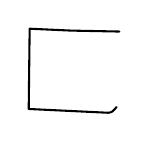
\begin{tikzpicture}[x=.012cm,y=-.012cm,line cap=round,line join=round]
 \draw[line width=.75pt] (98,4) -- (47,3) -- (3,1) -- (2,86) -- (86,90) .. controls (91,90) and (92,87) .. (95,84);
\end{tikzpicture}}
% archive sheet number: 20
